\documentclass{article} % Especially this!

%%%%%%%%%%%%%%%%%%%%%%%%%%%%%%%%%%%%%%%%%%%%%%%%%%%%%%%%

\usepackage[english]{babel}
\usepackage[utf8]{inputenc}
\usepackage[a4paper, total={6in, 8in}]{geometry}
\usepackage{amsmath}
\usepackage{amsthm}
\usepackage{amsfonts}
\usepackage{amssymb}
\usepackage[usenames,dvipsnames]{xcolor}
\usepackage{graphicx}
%\usepackage[siunitx]{circuitikz}
\usepackage{tikz}
\usepackage[colorinlistoftodos, color=orange!50]{todonotes}
\usepackage{hyperref}
\usepackage[numbers, square]{natbib}
\usepackage{fancybox}
\usepackage{epsfig}
\usepackage{soul}
\usepackage{listings}
\usepackage[framemethod=tikz]{mdframed}
\usepackage[shortlabels]{enumitem}
\usepackage[version=4]{mhchem}
\usepackage{multicol}
\usepackage{pgfplots}
\usepackage{version}
\pgfplotsset{compat=1.14}
\usepackage{graphicx}
\usepackage{subfig}

%%%%%%%%%%%%%%%%%%%%%%%%%%%%%%%%%%%%%%%%%%%%%%%%%%%%%%%

% SYNTAX FOR NEW COMMANDS:
%\newcommand{\new}{Old command or text}

% EXAMPLE:

\newcommand{\blah}{blah blah blah \dots}

\setlength{\marginparwidth}{3.4cm}


% NEW COUNTERS
\newcounter{points}
\setcounter{points}{100}
\newcounter{spelling}
\newcounter{english}
\newcounter{units}
\newcounter{other}
\newcounter{source}
\newcounter{concept}
\newcounter{missing}
\newcounter{math}
\newcounter{terms}
\newcounter{clarity}
\newcounter{late}

% COMMANDS
\newtheorem{theorem}{Theorem}

\newcommand{\late}{\todo{late submittal (-5)}
\addtocounter{late}{-5}
\addtocounter{points}{-5}}

\definecolor{pink}{RGB}{255,182,193}
\newcommand{\hlp}[2][pink]{ {\sethlcolor{#1} \hl{#2}} }

\definecolor{myblue}{rgb}{0.668, 0.805, 0.929}
\newcommand{\hlb}[2][myblue]{ {\sethlcolor{#1} \hl{#2}} }

\newcommand{\clarity}[2]{\todo[color=CornflowerBlue!50]{CLARITY of WRITING(#1) #2}\addtocounter{points}{#1}
\addtocounter{clarity}{#1}}

\newcommand{\other}[2]{\todo{OTHER(#1) #2} \addtocounter{points}{#1} \addtocounter{other}{#1}}

\newcommand{\spelling}{\todo[color=CornflowerBlue!50]{SPELLING (-1)} \addtocounter{points}{-1}
\addtocounter{spelling}{-1}}
\newcommand{\units}{\todo{UNITS (-1)} \addtocounter{points}{-1}
\addtocounter{units}{-1}}

\newcommand{\english}{\todo[color=CornflowerBlue!50]{SYNTAX and GRAMMAR (-1)} \addtocounter{points}{-1}
\addtocounter{english}{-1}}

\newcommand{\source}{\todo{SOURCE(S) (-2)} \addtocounter{points}{-2}
\addtocounter{source}{-2}}
\newcommand{\concept}{\todo{CONCEPT (-2)} \addtocounter{points}{-2}
\addtocounter{concept}{-2}}

\newcommand{\missing}[2]{\todo{MISSING CONTENT (#1) #2} \addtocounter{points}{#1}
\addtocounter{missing}{#1}}

\newcommand{\maths}{\todo{MATH (-1)} \addtocounter{points}{-1}
\addtocounter{math}{-1}}
\newcommand{\terms}{\todo[color=CornflowerBlue!50]{SCIENCE TERMS (-1)} \addtocounter{points}{-1}
\addtocounter{terms}{-1}}


\newcommand{\summary}[1]{
\begin{mdframed}[nobreak=true]
\begin{minipage}{\textwidth}
\vspace{0.5cm}
\begin{center}
\Large{Grade Summary} \hrule 
\end{center} \vspace{0.5cm}
General Comments: #1

\vspace{0.5cm}
Possible Points \dotfill 100 \\
Points Lost (Late Submittal) \dotfill \thelate \\
Points Lost (Science Terms) \dotfill \theterms \\
Points Lost (Syntax and Grammar) \dotfill \theenglish \\
Points Lost (Spelling) \dotfill \thespelling \\
Points Lost (Units) \dotfill \theunits \\
Points Lost (Math) \dotfill \themath \\
Points Lost (Sources) \dotfill \thesource \\
Points Lost (Concept) \dotfill \theconcept \\
Points Lost (Missing Content) \dotfill \themissing \\
Points Lost (Clarity of Writing) \dotfill \theclarity \\
Other \dotfill \theother \\[0.5cm]
\begin{center}
\large{\textbf{Grade:} \fbox{\thepoints}}
\end{center}
\end{minipage}
\end{mdframed}}

%#########################################################

%To use symbols for footnotes
\renewcommand*{\thefootnote}{\fnsymbol{footnote}}
%To change footnotes back to numbers uncomment the following line
%\renewcommand*{\thefootnote}{\arabic{footnote}}

% Enable this command to adjust line spacing for inline math equations.
% \everymath{\displaystyle}

%%%%%%%%%%%%%%%%%%%%%%%%%%%%%%%%%%%%%%%

\title{
\normalfont \normalsize 
\textsc{Physics of Complex Systems, 2021} \\ 
[10pt] 
\rule{\linewidth}{0.5pt} \\[6pt] 
\huge 
Simulation of a simple model of flocking
\rule{\linewidth}{2pt}  \\[10pt]
}
\author{Lorenzo Sani}
\date{\normalsize \today}

\begin{document}

\maketitle

\tableofcontents

%###############################################
\section{Abstract}
This short relation aims to show the results of the simulation of a simple model of flocking
in order to verify a theorem. At the same time, using the result of the simulation, it tries
to highlight the influence of the parameter of the model on the trend of the convergence.
%###############################################
\section{Introduction}
A common phenomena revealed by real complex systems is the emergence of a global 
behaviour in a system composed by many (sometimes identical) autonomous individuals or 
agents.
Physicists generally refer to emergence when the appearance of a global consensus cannot
be understood in the sense of the behaviours and laws of microscopic elements of a large
system; while refer to self-organization when the system reacts (or adapts) to external 
stimuli over time, and responds accordingly.
Examples of this behaviour can be found in many fields such economy, e.g. a 
common belief in a price system when activity takes place in a given market, or also
in biological systems, e.g. the way many animals moving together.
In this short relation it was simulated a simple model of flocking, where many birds,
with random initial positions and velocities, after some time assume the same velocity
and keep the same distances between each others.
%###############################################
\section {The Model}
This short study is based on a model presented in \cite{CuckerSmale} . The authors considered 
a population of birds moving in $\mathbf{E}=\mathbf{R}^3$, and, to model their dynamics, they
considered some empirical observations. In fact it has been observed that with some
initial conditions, on positions and velocities of birds, the state of the flock, i.e. 
the system of all the birds, converges to one in which the velocity of all the birds is 
the same. Keeping this observations in mind, the authors of \cite{CuckerSmale} postulated a 
model for the evolution of the flock. They found conditions under which the aimed convergence 
is reached. When these conditions are not satisfied the dispersion of birds is expected.
The model proposed postulates that every bird adjust its velocity by an additive term,
that is represented by the weighted average of the differences of its velocity with
those of other birds.
\begin{equation}
	\label{eq1}
	v_i(t+h)-v_i(t)=h\sum_{j=1}^k a_{ij}(v_j(t)-v_i(t))
\end{equation}
In \eqref{eq1} $h$ represents the time step; the matrix whose elements are $a_{ij}$  is 
the weighting matrix; $k$ is the number of birds in the system. At this point it is 
useful to remark the fact that the interaction between birds is global, i.e. every birds
interacts with all the others. This is clearly a strong simplification of reality.
For complex network theorists, the matrix $\lbrace a_{ij}\rbrace$ can represent the adjacency
matrix $A_x$, where the subscript $x$ is referred to the space variable, of the graph
representing the flock of birds. The graph represented by this adjacency matrix must be 
weighted, completely symmetric, and with non-zero constant diagonal.
Then it is reasonable to assumed that the weights are functions of the (visual) 
perception that every bird has of all the others. It is assumed a quite simple function 
of the distance between birds that is a non-increaing function 
$\eta:\mathbf{R}_+\rightarrow\mathbf{R}_+$ such that
\begin{equation}
	\label{eq2}
	a_{ij}=\eta(x_i,x_j)=\frac{H}{(1+\left\Vert x_i - x_j \right\Vert^2)^{\beta}}
\end{equation}
for some fixed values of $H>0$ and $\beta\geq0$. In \eqref{eq2} 
$\left\Vert \cdot \right\Vert$ represents the standard euclidean distance in our space 
$\mathbf{E}$. This function satisfies the properties requested by the graph.
We can write \eqref{eq1} in a more concise form by making use of some well-known 
properties of the adjacency matrix $A_x$, the degree matrix $D_x=diag(d_1,...,d_k)$, whose
elements are given by $d_i=\sum_{j\leq k}a_{ij}$, and the Laplacian of $A_x$ defined by
$L_x=D_x-A_x$. Then
\begin{align}
\label{eq3}
    v_i(t+h)-v_i(t)& = -h\sum_{j=1}^k a_{ij}(v_i(t)-v_j(t))\\
    & = -h(\sum_{j=1}^k a_{ij})v_i(t)+h\sum_{j=1}^k a_{ij}v_j(t))\nonumber\\
    & = -h\lbrack D_xv(t)\rbrack_i+h\lbrack A_xv(t)\rbrack\nonumber\\
    & = -h\lbrack L_xv(t)\rbrack_i\nonumber
\end{align}
In \eqref{eq3} is crucial to remark that the notation $A_xv(t)$ does not refer to a 
$k \times k$ matrix acting on $\mathbf{R}^k$, but $A_x$ maps $(v_1, \dotsb ,v_k)$ 
to $(a_{i1}v_1+ \dotsb +a_{ik}v_k)_{i\leq k}$. The same holds for $D_x$ and $L_x$.
Adding a simple natural equation for the evolution of the positions, the following
system is obtained
\begin{align}
\label{eq4}
    &x(t+h) = x(t) + hv(t)\\
    &v(t+h) = (Id -hL_x)v(t)\nonumber
\end{align}
The paper \cite{CuckerSmale} proposed also the continuous version of \eqref{eq4}, that
is simply obtained by letting $h$ tend to zero. The following system of differential 
equations is then given.
\begin{align}
\label{eq5}
    &\dot{x} = v\\
    &\dot{v} = -L_xv\nonumber
\end{align}
Finally the authors of \cite{CuckerSmale} proved the following theorem
\begin{theorem}
    Let $x_0,y_0\in \mathbf{E}$. Then, there exists a unique solution $(x(t),v(t))$ of 
    \eqref{eq5}, defined for all $t \in \mathbf{R}$, with initial conditions $x(0)=x_0$ and
    $v(0)=v_0$. If $\beta<1/2$ then, when $t\rightarrow\infty$ the velocities $v_i(t)$ tend
    to a common limit $\widehat{v}\in\mathbf{E}$ and the vectors $x_i-x_j$ tend to a limit 
    vector $\widehat{x_{ij}}$, for all $i,j\leq k$. The same happens if $\beta\geq1/2$ provided
    the initial values $x_0$ and $v_0$ satisfy a given, explicit, relation.
\end{theorem}
Looking a bit deeper inside the model, by following the graph theory view, it is notable that
the Laplacian $L_x$ gives us many information about the structure of the graph $G$ described
by the adjacency matrix $A$. $L_x$ is symmetric, positive semi-definite and can be used to 
build the energy function of the flock. Infact, by noting that
\begin{equation}
	\label{eq6}
	\forall v \in \mathbf{E}^3, L_x(v,...,v)=0,
\end{equation} and
\begin{equation}
	\label{eq7}
	\langle L_xv,v\rangle=\frac{1}{2}\sum_{i,j=1}^ka_{ij}\left\Vert v_i - v_j\right\Vert^2,
\end{equation}
using the standard euclidean scalar product, we can define 
\begin{equation}
	\label{eq8}
	E_x(v)=2\langle L_xv,v\rangle=\sum_{i,j=1}^ka_{ij}\left\Vert v_i - v_j\right\Vert^2
\end{equation}
Now it turns clear that the results of the theorem imply the fact that for $t\rightarrow\infty$ $E_x(v)=0$,
since all the birds are flying with the same velocity. The physical interpretation of the 
convergence in the theorem relies on the minimization of the energy of the flock. The question that
arises naturally is about how rapid is the convergence and how sharp is the critical value of $\beta=1/2$.
In \cite{CuckerSmale1} the authors give extended explanation on the 
discretization and assume, to maintain the validity of the theorem, one more constraint on
the function $\eta$ in \eqref{eq2}. They modified a bit the function to 
\begin{equation}
	\label{eq9}
	\eta(x_i,x_j)=\frac{H}{(\sigma^2+\left\Vert x_i - x_j \right\Vert^2)^{\beta}},
\end{equation}
where the new parameter $\sigma$ must be strictly positive, and they gave the constraint
\begin{equation}
	\label{eq10}
	H<\frac{\sigma^{2\beta}}{(k-1)\sqrt{k}},
\end{equation}
where $k$ is the number of birds in the flock.
Here $\sigma$ respresent a scaling parameter for the the space variables, while for the velocities
can be seen as an attenuation on their variation. In fact letting by $X(t)=\frac{x(t)}{\sigma}$ 
and $V(t)=\frac{v(t)}{\sigma}$, the system becomes
\begin{align}
\label{eq11}
    \dot{X_i} &= \frac{v_i}{\sigma} = V_i\\
    \dot{V_i} &= \frac{1}{\sigma^{2\beta}}\sum_{i,j=1}^k\frac{H}{(1+\left\Vert x_i - x_j \right\Vert^2)^{\beta}}(V_i - V_j)\nonumber
\end{align}
This shows that the dynamics for the space variables has not been changed by rescaling, while
the velocities show a modulation to their variation depending on the factor $\frac{1}{\sigma^{2\beta}}$.
Keeping this in mind, the speed of convergence it is expected to depend on the parameter $\sigma$ for the
velocities but not for the space variables.

%###############################################
\section {Simulation}
The model described above was simulated in its discretized version.
A simple program written in \verb|C++| was used to simulate the model in order to allow the
tuning of the parameters.
A modular function, that accepts different values for the parameters of the model, was used.
The function is responsible of keeping the necessary constraints for reaching the convergence.
It receives as arguments the number of birds $k$, the number of different values $r$
of $\beta\in[0,1]$ to simulate, the magnitude of the time step $h$, and the value of $\sigma$.
In every simulation $r=200$ and $h=1$ were fixed.
The interval for $\beta$ was choosen for being the most representative.
The initial conditions are taken randomly using the \Verb|mt19937| class provided by the 
\verb|random| standard library for both velocities and positions of the birds.
The simulation proceeds as the following pseudo-code explains
\begin{lstlisting}[language=C++]
do {
    computeAdjMatrix(); // compute the adjacency matrix
    computeAdjDegree(); // compute the degree matrix
    computeAdjLaplacian(); // compute the Laplacian matrix
    spatialDiffEq(); // apply the discrete differential equation for x
    velocityDiffEq(); // apply the discrete differential equation for v
} while (convergenceIsReached() || number_of_iterations > MAX_ITER)
\end{lstlisting}
A \verb|MAX_ITER| number was fixed to take the value of $10\times k$, where $k$ is the number
of birds, in order to optimize the iteration procedure. The entire code used can be found at \cite{repo}.
In \cite{repo} can be found also the \verb|Python| script used to read and elaborate the results
dumped by the \verb|C++| code.
%###############################################
\section {Results}
The focus of the simulation was in verifying the theorem and secondly
in underlying the dependence between the speed of the convergence
and some of the parameters, especially $\sigma$, the scaling factor, and $k$, the number of
birds in the flock.
Recalling that the theorem states that the velocities $v_i(t)$ tend to a common limit $\widehat{v}\in\mathbf{E}$
and the vectors $x_i-x_j$ tend to a limit vector $\widehat{x_{ij}}$, for all $i,j\leq k$, the procedure 
for checking the convergence is built in the following way. To check the convergence of the velocities,
it is measured the euclidean distancse between all the velocities, and the maximum of these $\epsilon_v$
is then retrieved. A value of $\epsilon_v$ close to zero means that the convergence is reached. To check the
convergence of the distances, the vector of the $x_{ij}=x_i-x_j$ with the largest components is retrieved,
then the scalar factor $\epsilon_x = \left\Vert x_{ij}^{(max)} \right\Vert$ is used to measure the convergence. 
A value of $\epsilon_x$
close to zero means that the convergence is reached. Since the simulation uses \verb|float| variables, the 
value closest to zero is represented by \verb|1.19e-7f|. In Fig.\ref{fig1} is shown the trend of the convergence for
both $\epsilon_x$ and $\epsilon_v$ in a standard setting with $\sigma=1$ and $k=100$. The shape of the curves
in Fig.\ref{fig1} are representative for every simulation, since this shape is a peculiarity of the model.
In Fig.\ref{fig2} is shown the trend of the $\epsilon_x$ and $\epsilon_v$, with different values
of the parameter $\sigma$ and the same $k=100$. While looking at this plot, one has to keep in mind that the
number of iterations has been fixed to 1000.
Finally in Fig.\ref{fig3}, two 3D plot are shown highlithing the dependence of $\epsilon_x$ and $\epsilon_v$
on the couple $\sigma$, $\beta$ at the same time and on the couple $k$, $\beta$ at the same time.
%###############################################
\section {Figures}
\begin{figure}[ht]
    \centering
    \subfloat[]{
        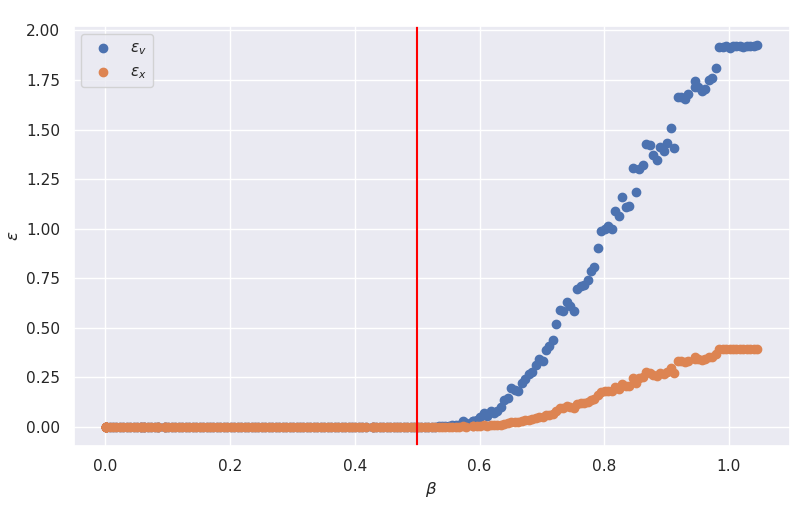
\includegraphics[width=0.45\textwidth, keepaspectratio]{images/N100_sigma1.png}
    }
    \subfloat[]{
        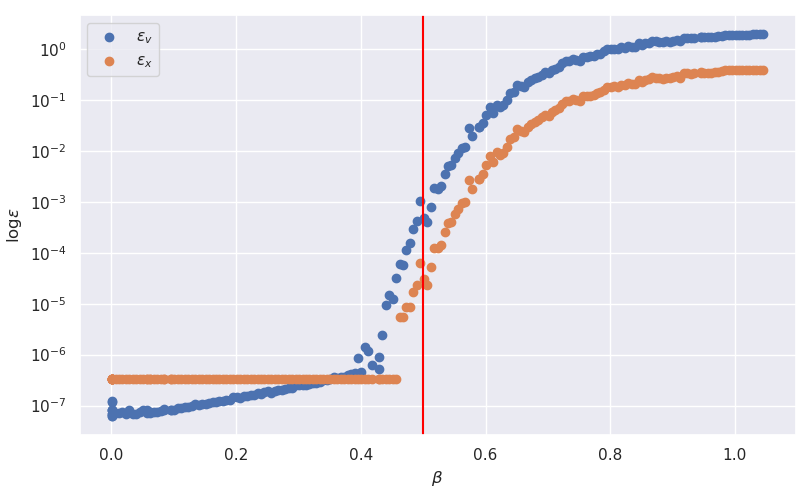
\includegraphics[width=0.45\textwidth, keepaspectratio]{images/N100_sigma1log.png}
    }
    \caption{Here is shown the tren of the convergence for the topical case with $\sigma=1$ 
        and $k=100$. In (a) are plotted $\epsilon_x$ and $\epsilon_v$ in linear scale, while 
        in (b) in logarithmic scale.}
    \label{fig1}
\end{figure}
\begin{figure}[hb]
    \centering
    \subfloat[]{
        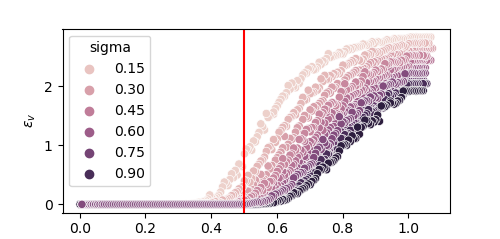
\includegraphics[width=0.45\textwidth, keepaspectratio]{images/N100_sigmaA.png}
    }
    \subfloat[]{
        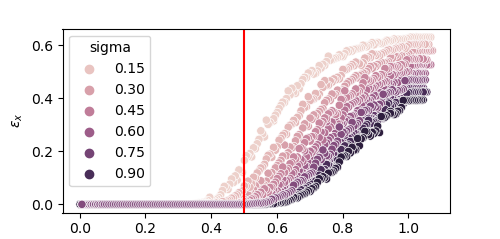
\includegraphics[width=0.45\textwidth, keepaspectratio]{images/N100_sigmaAX.png}
    }
    \caption{Here is shown the influence of the value of $\sigma$ on the trend of the 
        convergence. In (a) is plotted $\epsilon_v$, while in (b) $\epsilon_x$.}
    \label{fig2}
\end{figure}
\begin{figure}[ht]
    \centering
    \subfloat[]{
        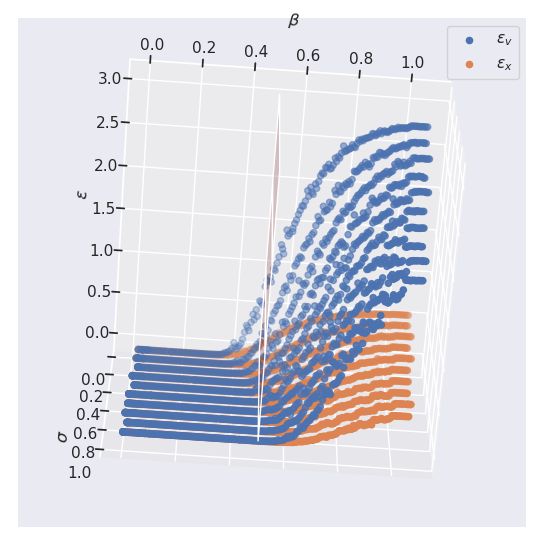
\includegraphics[width=0.45\textwidth, keepaspectratio]{images/N100_3d.png}
    }
    \subfloat[]{
        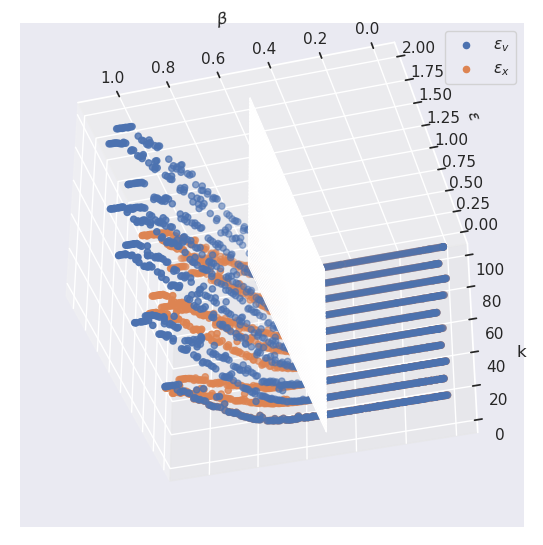
\includegraphics[width=0.45\textwidth, keepaspectratio]{images/sigma1_3d.png}
    }
    \caption{These 3D plots give a different view of the trend of the convergence 
        considering the parameter $\beta$, with $\sigma$ for the plot (a), and with 
        $k$ for the plot (b).}
    \label{fig3}
\end{figure}
%###############################################
\newpage
\section{Bibliography}
\begin{thebibliography}{90}
\bibitem{CuckerSmale}F. Cucker, S. Smale. "On the mathematics of emergence", The Mathematical Society of Japan and Springer 2007, Published online: 28 March 2007.
\bibitem{CuckerSmale1}F. Cucker, S. Smale. "Emergent Behaviour in Flocks", IEEE Transaction on Automatic Control, Vol. 52, No. 5, May 2007.
\bibitem{repo}\verb|https://github.com/relogu/PofCS_project|.
\end{thebibliography}

\newpage
\appendix
\renewcommand\thefigure{\thesection.\arabic{figure}}
\end{document} % NOTHING AFTER THIS LINE IS PART OF THE DOCUMENT